\documentclass[../main.tex]{subfiles}

\begin{document} %%%%%%%%%%%%%%%%%%%%%%%%%%%%%%%%%%%%%%%%%%%%%%%%%%%%%%%%%%%%%%%
\section{Supercised Learning}
    El Supercised Learning se puede clasificar en dos grandes grupos:
    
    \[ \schema {\schemabox{Supercised Learning}} { \schemabox{ \schema {\schemabox{Classification}} {\schemabox{Regresión logística \\ K-Nearest Neighbors (KNN) \\ Decision Trees \\ Random Forest}} \\ \schema {\schemabox{Regression}} {\schemabox{Linear Regression}} } } \]

    Existen métodos y algoritmos que se pueden usar en ambos problemas:
    \begin{table}[ht]
        \begin{center}
            \begin{tabular}{|l|c|c|}
                \hline
                \textbf{Supervised Learning} & \textbf{Classification} & \textbf{Regression} \\
                \hline
                Logistic Regression & \checkmark &  \\ \hline
                k-Nearest Neighbors (KNN)  & \checkmark & \checkmark \\ \hline
                Decision Trees & \checkmark & \checkmark \\ \hline
                Random Forest & \checkmark & \checkmark \\ \hline
                Support vector machine (SVM) & \checkmark &  \\ \hline
                Linear Regression &  & \checkmark \\
                \hline
            \end{tabular}
        \end{center}
        \caption{Cuadros}
    \end{table}
    
    
    \underline{Métricas Clasificación:}
        \begin{itemize}
            \item Precisión.
            \item Recall (exhaustividad).
            \item Valor-F ($F_1$)
        \end{itemize}
        
        Ver video 03b min 40. Matriz de confucion.

    \subsection{Classification}
        En el contexto del aprendizaje automático supervisado, la variable predictora (también conocida como variable independiente o característica) es una variable que se utiliza para predecir el valor de la variable objetivo (también conocida como variable dependiente o target). Las variables predictoras son los datos de entrada al modelo y la variable objetivo es el resultado que se desea predecir.
        
        \subsubsection{Regresión logística.}
            La regresión logística es un tipo de algoritmo de aprendizaje supervisado que se utiliza principalmente para resolver tareas de “clasificación” binarias, aunque contiene la palabra “regresión”. Se lo utiliza para predecir el resultado de una variable categórica (una variable que puede adoptar un número limitado de categorías) en función de las \textbf{variables predictoras} o independientes. Un ejemplo de clasificación podría ser la detección de spam: un programa de aprendizaje automático puede aprender a marcar el spam después de recibir ejemplos de correos electrónicos spam marcados (\textbf{variable objetivo} “target” sería una variable binaria que indica si un correo electrónico es spam o no) por los usuarios y ejemplos de correos electrónicos regulares no spam (también llamados “ham”).  Ejemplo Python \cite{regresión_logística_colab}. \\

            Tambien existe la regresion logistica multinomial, que es una generalizacion de la regresion logistica. En este caso la variable objetivo puede tomar mas de dos valores. Ver regresion\_logistica\_02.ipynb

        \subsubsection{K-Nearest Neighbors (KNN).}
            Se utiliza para clasificación y regresión.
            k vecinos más cercanos es un método de clasificación no paramétrico. Video de youtube \cite{knn_you_tube}.\\
            Se utiliza principalmente para la clasificación de datos no lineales y para resolver problemas de clasificación en los que los datos son muy complejos y desestructurados.\\
            
            Resumen:
            \begin{itemize}
                \item Es sensible a conjuntos de datos no balanceados.
                \item Es muy sensible aoutliers.
                \item La normalización de los datos de entrenamiento puede mejorar drásticamente su precisión
                \item Si se aplica en un comjunto de datos desbalanceado, puede ser que el algoritmo siempre prediga la clase mayoritaria. 
            \end{itemize}
    
        \subsubsection{Decision Trees}
            Los árboles de decisión son modelos ampliamente utilizados para tareas de clasificación y regresión. Esencialmente, aprenden una jerarquía de preguntas if/else, que conducen a una decisión. Estas preguntas son similares a las preguntas que podría hacer en un juego de 20 preguntas. Imagina que quieres distinguir entre los siguientes cuatro animales: osos, halcones, pingüinos y delfines. Su objetivo es llegar a la respuesta correcta haciendo la menor cantidad posible de preguntas si/si no. Puede comenzar preguntando si el animal tiene plumas, una pregunta que reduce sus posibles animales a solo dos. Si la respuesta es “sí”, puedes hacer otra pregunta que podría ayudarte a distinguir entre halcones y pingüinos. Por ejemplo, podría preguntar si el animal puede volar. Si el animal no tiene plumas, sus posibles opciones de animales son delfines y osos, y deberá hacer una pregunta para distinguir entre estos dos animales, por ejemplo, preguntar si el animal tiene aletas.

            % Cargamos una imagen y nombramos las figuras con un prefijo de la sección
            \begin{figure}[ht]
                \centering
                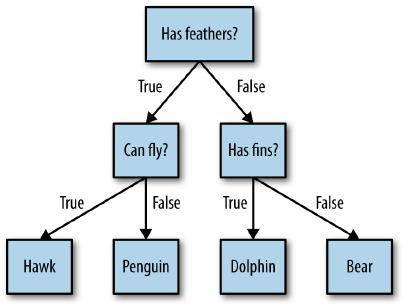
\includegraphics[width=0.5\textwidth]{./images/decision_trees_01.jpg}
                \caption{Ejemplo de un árbol de decisión.}
                \label{fig:tree_01}
            \end{figure}

            Existen varios algoritmos ID3, C4.5 y CART. Pagina buena \cite{tree_pag}:


            
            \paragraph{$\bullet$ ID3 - Iterative Dichotomiser 3:}
                Genera un árbol de decision a partir de un conjunto de ejemplos.\\
                Este algoritmo usa las metricas de \textit{entropía} y \textit{ganancia de la información}. Cuando se usa la librería sklearm \textit{sklearn.tree.DecisionTreeClassifier} en el parámetro \textit{criterion} colocar \textit{entropy}.
                
                \begin{itemize}
                    \item Un nodo principal llamado raíz en la parte superior.
                    \item Nodos terminales. como su nombre lo indica, son nodos donde termina el flujo y que ya no son raiz de ningún otro nodo. Estos nodos terminales deben contener una respuesta, o sea, la clasificación a que pertenece el objeto que ha conducido hasta él.
                    \item Los demás nodos representan preguntas con respecto al valor de uno de los atributos.
                    \item Las líneas nodos representan preguntas con respecto al valor de uno de sus atributos.
                    \item Las líneas representa las posibles respuestas que los atributos pueden tomar.
                \end{itemize}
        
                \textbf{Algoritmo básico}
                \begin{enumerate}
                    \item Calcular la entropía para todas las clases.
                    \item Calcular la entropía para cada valor posible de cada atributo.
                    \item Seleccionar el mejor atributo basado en la reducción de la entropía. usando el calculo de la ganancia de la información.
                    \item Iterar, para cada sub-nodo, Excluyendo el nodo raíz, que ya fue usado.
                \end{enumerate}
            
                \paragraph{$\bullet$ C4.5:}
                Utiliza la metrica \textit{gini}.
            
                \begin{enumerate}
                    \item Mitiga el sobreajuste por que emplea inherentemente el proceso de poda de un solo paso.
                    \item Funciona para datos discretos y continuos.
                    \item Es útil para datos incompletos.
                \end{enumerate}
            
            \underline{\textbf{Metricas:}}
            \begin{itemize} 
                \item 
                    \textbf{Entropía:} \\
                    La medida del desorden o la medida de la pureza. Básicamente, es la medida de la impureza o aleatoriedad de los datos.\\

                    Para calcular la entropia de $n$ clases se utiliza la fórmula:
                    \begin{equation}
                        H(S) = \sum_{i=1}^{n} -p_i \cdot  \log_2(p_i)
                    \end{equation}
                
                    Dónde:
                    \begin{itemize}
                        \item $S$: es una lista de valores posibles.
                        \item $p_i$: es la probabilidad de los valores.
                        \item $i$: cada uno de los valores.
                    \end{itemize}
                
                    Importante:
                    \begin{itemize}
                        \item Para una muestra homogénea la entropia es igual a cero 0. Si no existe aleatoriedad, es decir, una moneda cargada.
                        \item La máxima entropía viene dada por $\log_2(n)$, $n$ son los posibles valores de salida. Si $n=2$ (true o false) entonces, la máxima entropía es 1. O sea es la máxima incertidumbre, ejemplo moneda equilibrada.
                    \end{itemize}

                \item 
                    \textbf{Ganancia de la Información:}
                    La ganancia de la información se aplica a cuantificar qué característica, de un conjunto de datos dados, proporciona la máxima información sobre la clasificación.
            \end{itemize}               
        
        \subsubsection{Random Forest - Bosques aleatorios.}
            Usa una técnica, o meta-algoritmo llamado Bootstrap aggregating. Se crean m tablas reducidas en atributos y para cada una de ellas entrenamos un árbol.
        
        \subsubsection{Support Vector Machines (SVM)}
            Es un algoritmo de aprendizaje supervisado que se puede utilizar para problemas de clasificación o regresión. El algoritmo SVM utiliza un hiperplano para separar los datos en clases. El hiperplano se selecciona de tal manera que maximiza la distancia entre los puntos de datos de las clases. El hiperplano se puede utilizar para clasificar nuevos puntos de datos.\\
            
            \textbf{Ventajas:}
            \begin{itemize}
                \item Efectivo en espacios de alta dimensión.
                \item Efectivo en casos en que el número de dimensiones es mayor que el número de muestras.
                \item Utiliza un subconjunto de puntos de entrenamiento en la función de decisión (llamados vectores de soporte), por lo que también es eficiente en memoria.
                \item Versátil: se pueden especificar diferentes funciones del núcleo para la función de decisión. Se proporcionan núcleos comunes, pero también es posible especificar núcleos personalizados.
            \end{itemize}
            
            \textbf{Desventajas:}
            \begin{itemize}
                \item Si el número de características es mucho mayor que el número de muestras, evite el exceso de ajuste al elegir las funciones del núcleo y el término de regularización es crucial.
                \item Los SVM no proporcionan directamente estimaciones de probabilidad, estas se calculan utilizando una validación cruzada de cinco veces.
            \end{itemize}
            
            \textbf{Parámetros:}
            \begin{itemize}
                \item \textbf{C:} Parámetro de regularización. El parámetro C controla el comercio entre el ajuste de los datos de entrenamiento y la suavidad de la superficie de decisión. Un C alto significa que el clasificador intentará ajustar los datos de entrenamiento lo mejor posible, mientras que un C bajo significa que el clasificador buscará una superficie de decisión que esté lo más suave posible.
                \item \textbf{kernel:} Especifica el tipo de kernel que se utilizará en el algoritmo. Debe ser uno de 'lineal', 'poli', 'rbf', 'sigmoid', 'precomputed' o una llamada a un kernel personalizado.
                \item \textbf{degree:} Grado de la función del núcleo polinomial ('poly'). Ignorado por todos los demás núcleos.
                \item \textbf{gamma:} Coeficiente para 'rbf', 'poly' y 'sigmoide'. Si gamma es 'auto', entonces 1 / n\_features se utilizará en su lugar.
                \item \textbf{coef0:} Término independiente en función del núcleo. Solo es significativo en 'poly' y 'sigmoide'.
                \item \textbf{probability:} Habilita la estimación de la probabilidad. Debe estar habilitado antes de llamar a fit, y se basa en una validación cruzada de cinco veces. Deshabilitarlo puede acelerar el cálculo cuando se usa svm en grandes conjuntos de datos.
                \item \textbf{shrinking:} Habilita o deshabilita el encogimiento heurístico de la función de decisión. Debe estar habilitado para el uso de la validación cruzada de probabilidad. Deshabilitarlo puede dar una pequeña ganancia de rendimiento.
            \end{itemize}

            Linealmente separable: es un conjunto de datos que se puede separar en dos grupos distintos de manera que no haya puntos de datos que se superpongan entre los dos grupos.\\
            
    \subsection{Regresión}
        Los modelos que existe para la regresión son:
        \begin{itemize}
            \item Regresión lineal y multiple: \textit{sklearn.linear\_model.Regresión Lineal}
            \item Regresión polinómica: \textit{sklearn.preprocessing.PolynomialFeatures}
        \end{itemize}

        \subsubsection{Regresión Lineal}
            La regresión lineal es un método estadístico que se utiliza para estudiar la relación entre una variable dependiente (también conocida como variable objetivo) y una o más variables independientes (también conocidas como variables predictoras). El objetivo de la regresión lineal es encontrar la línea (recta) que mejor se ajuste a los datos y pueda utilizarse para hacer predicciones.
        
           \begin{equation}
                y = a \cdot x + b
           \end{equation}
            
        \subsubsection{Regresión Lineal Múltiple}
            Consiste en predecir una respuesta numérica $y$ en base a múltiples variables predictoras $x_1, x_2, ..., x_n $, suponiendo una relación lineal. 
		
		\begin{equation}
			y = a_1 \cdot x_1 + a_2 \cdot x_2 + ... + a_n \cdot x_n + b
		\end{equation}
		
	\subsection{Métricas Regresión:}
        Las métricas de evaluación son medidas utilizadas para evaluar el rendimiento de un modelo de aprendizaje automático. En el caso de los problemas de regresión en el aprendizaje supervisado, estas métricas nos ayudan a determinar qué tan bien nuestro modelo está haciendo predicciones cuantitativas, como valores continuos.\\
    
        \underline{Metricas para la regresión:}
        \begin{itemize}
            \item Raíz del error cuadrático medio \textbf{(RMSE)}.
            \item Error absoluto medio \textbf{(MAE)}.
            \item Error cuadratico medio \textbf{(MSE)}.
            \item Suma Residual de los cuadrados \textbf{RSS}.
        \end{itemize}
    
        \underline{Para cada una de las métricas:}
        \begin{itemize}
            \item $m:$ número de instancias
            \item $h:$ Funcion hipotesis, es el modelo entrenado. En este caso regresion lineal.
            \item $x:$ Todos los valores de entrada, todas las columnas.
        \end{itemize}
        
        \begin{definition} (Error cuadrático medio \textbf{(MSE)})
            \begin{equation}
                MSE(X, h) = \frac{1}{m} \cdot RSS = \frac{1}{m} \cdot \sum_{i=1}^{m} (h(x^{(i)}) - y^{(i)})^2
            \end{equation}
        \end{definition}
        
        \begin{definition} (Error absoluto medio \textbf{(MAE)}
            \begin{equation}
                MAE(X, h) = \frac{1}{m} \cdot \sum_{i=1}^{m} |h(x^{(i)} - y^{(i)}|
            \end{equation}
        \end{definition}

        \begin{definition} (Raíz del error cuadrático medio \textbf{(RMSE)}
            \begin{equation}
                RMSE(X, h) = \sqrt{\frac{1}{m} \cdot \sum_{i=1}^{m}(h(x^{(i)}-y^{(i)}))^2}
            \end{equation} 
        \end{definition}


		          
\end{document} %%%%%%%%%%%%%%%%%%%%%%%%%%%%%%%%%%%%%%%%%%%%%%%%%%%%%%%%%%%%%%%